%\documentclass[handout]{beamer}
\documentclass{beamer}
\usepackage{etex}

\let\latexput\put
\usepackage{pictex}
\let\pictexput\put
\let\put\latexput

\begin{document}
\title{Detecting Adaptive Evolution}
\author{Alan R. Rogers}
\date{\today}

\frame{\titlepage}

\begin{frame}
  \frametitle{Conventional wisdom}

  Something must have happened to weaken the selective pressure
  drastically.  We cannot escape the conclusion that man's evolution
  towards manness suddenly came to a halt.\newline\mbox{}\hfill
  ---Ernst Mayr 1963

\medskip

  Natural selection has almost become
  irrelevant in human evolution.  There's been no biological change in
  humans in 40,000 or 50,000 years.  Everything we call culture and
  civilization we've built with the same body and brain.\newline
\mbox{}\hfill  ---Stephen Jay Gould 2000

\medskip

Certainly, human nature is fixed. It's universal and
unchanging\linebreak---common to every baby that's born, down through
the history of our species.\newline\mbox{}\hfill ---Helena Cronin
2000 %\emph{Getting Human Nature Right}.

\medskip
\pause

\textbf{Is this really true? How could we know?}
\end{frame}

\begin{frame}
\frametitle{Signatures of selection}
\begin{itemize}
\item High proportion of functional changes
\item Reduction of gene diversity
\item Population differences
\item Excess of singletons
\item Common allele on long LD block
\item Singleton density
\end{itemize}
\end{frame}

\begin{frame}
\frametitle{Time scale for signatures of selection}
\includegraphics[width=\textwidth]{scaletree.jpg}
\end{frame}

\begin{frame}
\frametitle{PRM1 gene}
\includegraphics[width=\textwidth]{prm1.jpg}\\
\begin{itemize}
\item compacts sperm DNA
\item 13/14 human-chimp diffs are non-synonymous (6 shown here)
\end{itemize}
\end{frame}

%\begin{frame}
%\frametitle{Proportion of functional changes at FOXP2 locus}
%\begin{itemize}
%\item Mutations at FOXP2 cause problems with language.
%\item Few amino acid changes within mammals $\Rightarrow$ strong
%  selective constraint. 
%\item Two mutations on human lineage, neither synonymous
%$\Rightarrow$ selection 
%\end{itemize}
%\mbox{} \hfill (Enard et al 2002)
%\end{frame}
%
%\begin{frame}
%\frametitle{Evolution of FOXP2}
%\includegraphics[width=\textwidth]{foxp2tree.jpg}\\
%\small Vertical bars separate nucleotide substitutions; gray
%indicates amino-acid changes. \hfill (Enard et al 2002)
%\end{frame}

\begin{frame}
\frametitle{Melanocortin 1 receptor (MC1R) locus}
\begin{itemize}
\item Affects color of skin and hair.
\item human-chimp $K_a/K_s = 0.63$: large for a functional protein
  $\Rightarrow$ weak selective constraint
\item Yet $K_a/K_s = 0$ among Africans.
\item On the other hand, $K_a/K_s \gg 0$ among Europeans
\end{itemize}
\end{frame}

\begin{frame}
\frametitle{Hypothesis}
\begin{itemize}
\item Before loss of body hair: weak selective constraint on MC1R
\item After loss: constraint strong w/i Africa; weak w/i Europe
\item Selective sweep at loss of body hair
\item Neutral diversity within Africa accumulated since the sweep.  
\end{itemize}
\end{frame}

\begin{frame}
\frametitle{Time required to generate African neutral $\hat\pi$}
{\centering% -*-latex-*-
\let\put\pictexput
\mbox{\beginpicture
\linethickness=1.5pt
\setplotsymbol({\large .})
\valuestolabelleading=.4\baselineskip
\setcoordinatesystem units <.04in, 1.7in>
\setplotarea x from 0.0 to 46.3, y from 0 to 1
\axis left label {\Large $\pi$} /
\axis bottom label {\large Millions of Years}
  ticks withvalues 0 0.5 1 1.5 / at 0 12.006 24.012 36.018 / /
\setdashes
\putrule from 0 0.6678 to 46.3 0.6678
\setdots
\putrule from 9.257673744 0 to 9.257673744 0.3339
\putrule from 0 0.3339 to 9.257673744 0.3339
%
\putrule from 18.5153474 0 to 18.5153474 0.50085
\putrule from 0 0.50085 to 18.5153474 0.50085
%
\putrule from 27.77302123 0 to 27.77302123 0.584325
\putrule from 0 0.584325 to 27.77302123 0.584325
%
\put {$\hat\pi = .67$} [b] <0pt,2pt> at 35, 0.67
\put {$\leftarrow$3 half-lives = 1.2 myr} [bl]
     at 27.77302123 0.05
%
\setsolid
% N = Infinity
\setbox0=\hbox{$\searrow$}%
\put {\raise \ht0 \hbox{$N=\infty$}$\searrow$} [br]
     at 18 0.9
\plot
0 0
20 1
/
% x: 2*u*t, where t is time in years
% y: mean pairwise difference
% Calculations assume that N=13906
\setbox0=\hbox{$\nwarrow$}%
\put {$\nwarrow$\lower \ht0 \hbox{$N=14000$}} [tl]
     at 31.24464888 0.6034319757
\plot
0 0
1.157209218 0.05542469995
2.314418436 0.1062493739
3.471627654 0.1528558054
4.628836872 0.1955940915
5.78604609 0.2347852727
6.943255308 0.2707237443
8.100464526 0.3036794681
9.257673744 0.3339
10.41488296 0.36161235
11.57209218 0.3870246869
12.7293014 0.4103279027
13.88651062 0.4316970458
15.04371983 0.4512926364
16.20092905 0.4692618722
17.35813827 0.485739734
18.51534749 0.50085
19.67255671 0.514706175
20.82976592 0.5274123435
21.98697514 0.5390639513
23.14418436 0.5497485229
24.30139358 0.5595463182
25.45860279 0.5685309361
26.61581201 0.576769867
27.77302123 0.584325
28.93023045 0.5912530875
30.08743967 0.5976061717
31.24464888 0.6034319757
32.4018581 0.6087742614
33.55906732 0.6136731591
34.71627654 0.618165468
35.87348576 0.6222849335
37.03069497 0.6260625
38.18790419 0.6295265437
39.34511341 0.6327030859
40.50232263 0.6356159878
41.65953185 0.6382871307
42.81674106 0.6407365795
43.97395028 0.642982734
45.1311595 0.6450424668
46.28836872 0.64693125
/
% N = 30000
% Calculations assume that N=30000
\setbox0=\hbox{$\nearrow$}%
\put {$\nwarrow$\lower \ht0 \hbox{$N=30000$}} [tl]
     at 31.2525 0.9537101618
\plot
0 0
1.1575 0.05672796537
2.315 0.1112222823
3.4725 0.1635709
4.63 0.2138583048
5.7875 0.2621656565
6.945 0.3085709192
8.1025 0.353148987
9.26 0.3959718053
10.4175 0.4371084865
11.575 0.4766254219
12.7325 0.5145863886
13.89 0.5510526523
15.0475 0.5860830666
16.205 0.6197341677
17.3625 0.6520602656
18.52 0.6831135321
19.6775 0.7129440845
20.835 0.7416000669
21.9925 0.7691277276
23.15 0.7955714941
24.3075 0.8209740443
25.465 0.8453763758
26.6225 0.8688178721
27.78 0.8913363657
28.9375 0.9129681996
30.095 0.9337482859
31.2525 0.9537101618
32.41 0.9728860441
33.5675 0.9913068812
34.13032585 1
/
\endpicture}
\let\put\latexput
\\[1ex]}
\small Trajectories of $\pi$ following a selective
sweep.  Dotted lines show the half-lives 
when $N=14,000$; the dashed line shows $\hat\pi$, the
observed value of $\pi$ in Africa.
\end{frame}

%\begin{frame}
%\frametitle{Kell}
%\includegraphics[width=\textwidth]{kell.jpg}
%\end{frame}

%\begin{frame}
%\frametitle{Duffy}
%\includegraphics[width=\textwidth]{duffy.jpg}
%\end{frame}

\begin{frame}
\frametitle{Duffy map}
\includegraphics[width=\textwidth]{duffymap.jpg}
\end{frame}

\begin{frame}
\frametitle{How a ``hard'' selective sweep generates LD}
\centering\includegraphics[height=0.8\textheight]{sweep-lzw.pdf}\\
\end{frame}

\begin{frame}
\frametitle{DNA sequences from region of human lactase gene}
%DNA sequences near human lactase gene, typed in a
%European sample.  Columns are
%nucleotide sites.  Top row (the
%reference sequence) shows common state at each site. Capital
%\texttt{A} is lactase persistance
%allele\cite{Bersaglieri:AJH-74-1111}.  Numbered rows represent
%individual chromosomes. Dots indicate identity with top row.  60
%chromosomes identical to reference sequence were omitted to save
%space. From HapMap release r23.}\label{tab.lctseq}
%
\tiny
\centering
\ttfamily
\begin{tabular}{cc}
  &cgcttcaggcattcctatctaaacagaccaacgtaAgggtacaatgcctaacccagacgtttcaactct\\
20&.....................................................................\\
21&.....................................................................\\
22&.....................................................................\\
23&.....................................................................\\
24&.....................................................................\\
25&.....................................................................\\
26&.....................................................................\\
27&..................t..................................................\\
28&..................t..................................................\\
29&..................................................c..................\\
37&...................................G..a.gt.....t.........gac.c.tgtct.\\
38&...ccgga....gat..at..gg..c.....tc.gGaaa.g..ccttt...tg......c...t.t...\\
39&...ccgga....gat..at..gg..c.....tc.gGaaa.g..ccttt...tg......c...t.t...\\
40&..tcc...agtag.t.cat..g.....t..ttccgG..a.gt.....t.........gac.c.tgtct.\\
41&..tcc...agtag.t.cat..g.....t.gttccgG..a.gt.....t.........gac.c.tgtct.\\
42&..tcc...agtag.t.cat..g.....t.gttccgG..a.gt.....t.........gac.c.tgtct.\\
43&..tcc...agtag.t.cat..g.....t.g.tc.gG..a.gt.....t.........gac.c.tgtct.\\
44&..tcc...agtag.t.cat..g.....t..ttc.gG..acgt.....t.........gac.c.tgtct.\\
45&..tcc...agtag.t.cat..g.....t.gttc.gG..a.gt.....t.........gac.c.tgtct.\\
46&...ccgga....gat..at..gg..c.....tc.gGaaa.g..ccttt...tg......cg.gt.t..c\\
47&..tcc...agtag.t.cat..g.....t.gttccgG..a.gt.....t.........gac.c.tgtct.\\
48&..tcc...agtag.t.cat..g.....t.gttccgG..a.gt.....t.........gac.c.tgtct.\\
49&..tcc...agtag.t.cat..g.....t.gttccgG..a.gt.....t.........gac.c.tgtct.\\
50&tatccgga....g.tc.atcgg.tc.g.tg.tc.gG..a.g.g....tg....ggt...cg.gt.t..c\\
51&ta.ccgga....g.t..atcgg.tc.g.tg.tc.gG..a.g.g....tg....ggt...cg.gt.t..c\\
52&ta.ccgga....g.t..atc.g.tc.g.tg.tc.gG..a.g.g....tg....ggt...cg.gt.t..c\\
53&ta.ccgga....g.t..atcgg.tc.g.tg.tc.gG..a.g.g....tg....ggt...cg.gt.t..c\\
\end{tabular}
\end{frame}

\begin{frame}
\frametitle{Huge block of LD around lactase allele in Europe}
\centering\includegraphics[height=0.8\textheight]{lactaseldblock.jpg}\\
\end{frame}

%%%%%%%%%%%%%%%%%%%%%%%%%%%%%%%%%%%%%%%%%%%%%%%%%%%%%

\begin{frame}
\frametitle{Idea behind Extended Haplotype Homozygosity (EHH)}
\begin{columns}
\column{0.5\textwidth}
%DNA sequences near human lactase gene, typed in a
%European sample.  Columns are
%nucleotide sites.  Top row (the
%reference sequence) shows common state at each site. Capital
%\texttt{A} is lactase persistance
%allele\cite{Bersaglieri:AJH-74-1111}.  Numbered rows represent
%individual chromosomes. Dots indicate identity with top row.  60
%chromosomes identical to reference sequence were omitted to save
%space. From HapMap release r23.}\label{tab.lctseq}
%
\tiny
\centering
\ttfamily
\begin{tabular}{c@{\hspace{1.5ex}}c}
  &ctaaacagaccaacgtaAgggtacaatgcctaacccagacgttt\\
20&............................................\\
21&............................................\\
22&............................................\\
23&............................................\\
24&............................................\\
25&............................................\\
26&............................................\\
27&t...........................................\\
28&t...........................................\\
29&................................c...........\\
37&.................G..a.gt.....t.........gac.c\\
38&t..gg..c.....tc.gGaaa.g..ccttt...tg......c..\\
39&t..gg..c.....tc.gGaaa.g..ccttt...tg......c..\\
40&t..g.....t..ttccgG..a.gt.....t.........gac.c\\
41&t..g.....t.gttccgG..a.gt.....t.........gac.c\\
44&t..g.....t..ttc.gG..acgt.....t.........gac.c\\
45&t..g.....t.gttc.gG..a.gt.....t.........gac.c\\
46&t..gg..c.....tc.gGaaa.g..ccttt...tg......cg.\\
47&t..g.....t.gttccgG..a.gt.....t.........gac.c\\
48&t..g.....t.gttccgG..a.gt.....t.........gac.c\\
49&t..g.....t.gttccgG..a.gt.....t.........gac.c\\
50&tcgg.tc.g.tg.tc.gG..a.g.g....tg....ggt...cg.\\
51&tcgg.tc.g.tg.tc.gG..a.g.g....tg....ggt...cg.\\
\end{tabular}

\column{0.55\textwidth}
\textcolor{blue}{Upper half:} pairs of chromosomes are identical
at most sites

\bigskip\pause

\textcolor{blue}{Lower half:} pairs identical at fewer sites

\bigskip\pause

This idea underlies EHH.
\end{columns}
\end{frame}

\begin{frame}
\frametitle{Extended haplotype homozygosity (EHH)}

\begin{itemize}
\item Select chromosomes that carry allele $A$ at focal site.
\item Within this set, calculate the fraction of pairs that are
  identical at another site, $x$ base-pairs away.  This is
  $\hbox{EHH}(x)$.
\item Do the same for chromosomes that \emph{don't} carry $A$.
\item \textcolor{blue}{relative EHH} is the ratio of the two.
\end{itemize}
\end{frame}

\begin{frame}
\frametitle{Decay of EHH with distance along chromosome}
\includegraphics[width=\textwidth]{voight-ehhdecay.png}
\end{frame}

\begin{frame}
\frametitle{EHH at candidate locus: SPAG4}
 \includegraphics[width=\textwidth]{voight-spag4.png}
\end{frame}

\begin{frame}
\frametitle{iHS, the integrated haplotype score}
\begin{columns}
\column{0.5\textwidth}
 \includegraphics[width=\linewidth]{voight-spag4.png}
\column{0.5\textwidth}
iHS is a normalized measure of the area between the two curves.
\end{columns}
\end{frame}

\begin{frame}
\frametitle{EHH at candidate locus: SNTG1}
 \includegraphics[width=\textwidth]{voight-sntg1.png}
\end{frame}

\begin{frame}
\frametitle{EHH at candidate locus: NCOA1}
 \includegraphics[width=\textwidth]{voight-ncoa1.png}
\end{frame}

\begin{frame}
\frametitle{Huge block of LD around lactase allele in Europe}
{\centering\includegraphics[width=\textwidth]{lac.png}\\}
\mbox{}\hfill\small (Nathan Harris)\\
\end{frame}

\begin{frame}
\begin{columns}
\column{0.6\textwidth}
 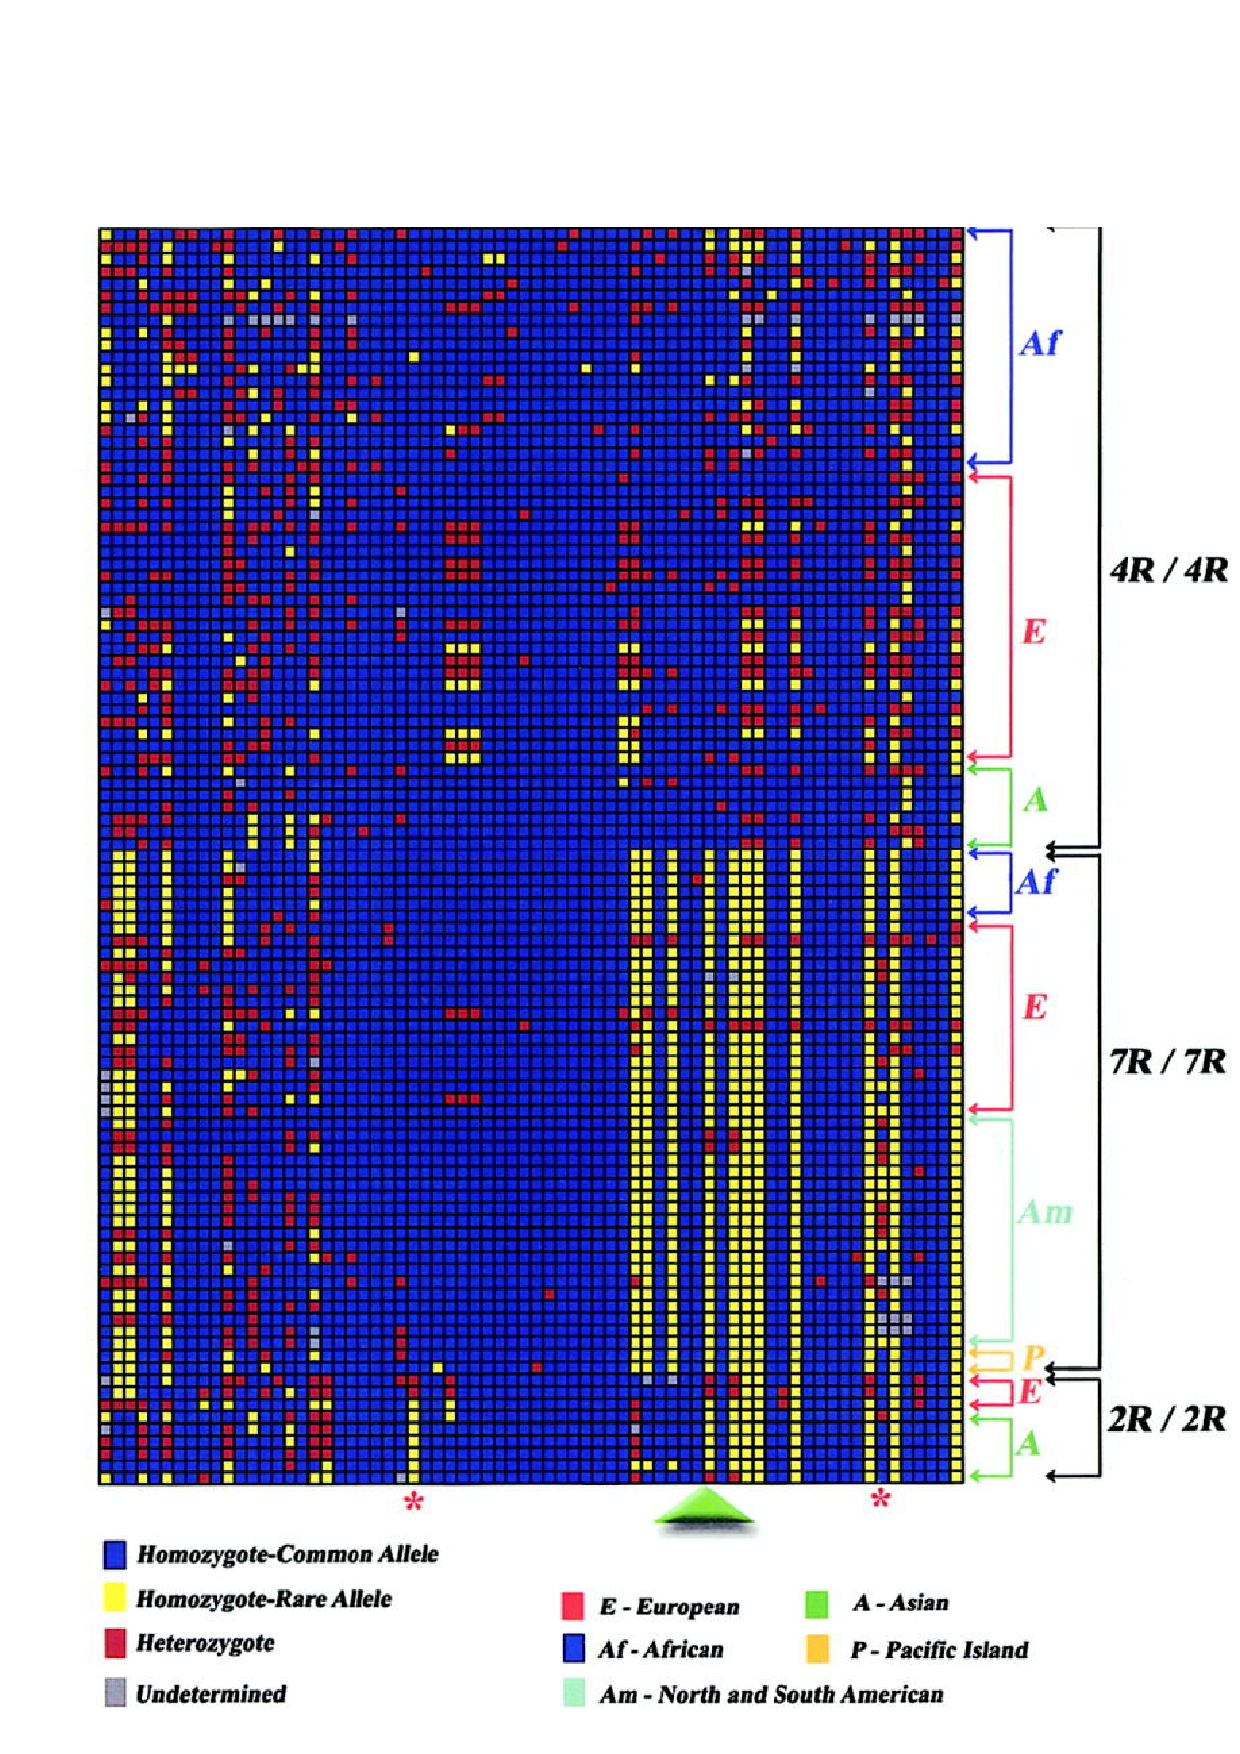
\includegraphics[width=\textwidth]{drd4-polymorph.pdf}
\column{0.4\textwidth}
\raggedright
Signature of an ongoing selective sweep at DRD4
\begin{itemize}
\item Sweeping allele is
\begin{itemize}
\item common
\pause
\item has low diversity over large region
\end{itemize}
\pause
\item High LD over large region
\end{itemize}
\end{columns}
\end{frame}

\begin{frame}
\frametitle{Linkage disequilibrium at G6PD}
\framesubtitle{Left: LD plot; right: haplotype plot}
 \includegraphics[width=\textwidth]{g6pd-ld.pdf}
\end{frame}

\begin{frame}
\frametitle{Study of Voight et al (2006)}
\begin{itemize}
\item 800,000 SNPs in 309 people
\item 431 sweeping loci
\item Most sweeps started w/i past 10,000 years
\end{itemize}
\end{frame}

\begin{frame}
\frametitle{LD on human chromosome 2 (Voight et al 2006)}
\includegraphics[width=\textwidth]{voight-loci.pdf}
\end{frame}

\begin{frame}
\begin{columns}
\column{0.65\textwidth}
 \includegraphics[height=0.9\textheight]{voight-venn.pdf}
\column{0.35\textwidth}
Voight et al (2006): 431 sweeping loci.

\medskip

{\color{red} ASN: Asia\\
\color{green} YRI: Africa\\
\color{blue} CEU: Europe.}

\medskip

\pause
Most are sweeping w/i only one continent.
\end{columns}
\end{frame}

\begin{frame}
\frametitle{IBD5}
{\centering\includegraphics[height=0.8\textheight]{Huff-IBD5-hitch.png}\\}
\mbox{}\hfill\footnotesize(Huff et al. 2012)
\end{frame}

\begin{frame}
\frametitle{IBD5 and inflammatory bowel disease}
\begin{itemize}
\item IBD5 is a 250~kb haplotype associated with Crohn's disease.
\item Within this region, variant 503F of the OCTN1 gene covaries with Crohn's.
\item OCTN1 transports the antioxidant ergothioneine.
\item Why should such a gene cause Crohn's disease?
\end{itemize}
\end{frame}

\begin{frame}
\frametitle{Ergothioneine (ET)}
\begin{itemize}
\item An antioxidant, synthesized by fungi, and present in most plants
and animals.
\item Low in wheat, barley, lentils, and peas---foods domesticated
early in Middle East.
\item Early farmers would have lacked ET.
\end{itemize}
\end{frame}

\begin{frame}
\frametitle{The OCTN1 protein}
\begin{itemize}
\item Transports ergothioneine (ET).
\item The 503F mutation increases rate of ET transport by 50\%.
\item Highly conserved in evolution, suggesting strong selection.
\item Highly specific to ET.
\item Common in Middle East and Europe; rare elsewhere.
\item LD extent suggests that 503F mutated 7,750--19,025~y ago.
\end{itemize}
\end{frame}

\begin{frame}
\frametitle{Distribution of early farming (A) and 503F (B)}
{\centering\includegraphics[width=\textwidth]{Huff-IBD5-map.png}\\}
\end{frame}

\begin{frame}
\frametitle{503F sits on a long LD block}
{\centering\includegraphics[width=\textwidth]{Huff-IBD5-bifur-503F.png}\\}
\end{frame}

\begin{frame}
\frametitle{503L sits on a short LD block}
{\centering\includegraphics[width=\textwidth]{Huff-IBD5-bifur-503L.png}\\}
\end{frame}

%\begin{frame}
%\frametitle{IBD5}
%{\centering\includegraphics[width=\textwidth]{Huff-IBD5-expression.png}\\}
%\end{frame}

\begin{frame}
  \frametitle{Selective sweep reduces diversity at linked loci}
\begin{columns}
  \column{0.5\textwidth}
  \includegraphics[width=\linewidth]{hetztrough}

  \bigskip

  \raggedright
  Horizontal axis: distance from selected locus in units of $c/s$,
  where $c$ is recombination rate and $s$ is selection coefficient.

  \column{0.5\textwidth}
  \raggedright

  Vertical: surviving fraction of neutral heterozygosity at linked
  loci.

  \bigskip

  Reduction is appreciable at loci for which $c < s/10$. (Gillespie,
  2004, Fig.~4.4)

  \bigskip

  Purifying selection (against deleterious mutations) also reduces
  linked variation.
\end{columns}  
\end{frame}  

\begin{frame}
\frametitle{Gene diversity vs.\ distance from exons, scaled by
  human-rhesus divergence}
{\centering\includegraphics[width=\linewidth]{Hernandez-loDiversity.png}\\}
\mbox{}\hfill\small Hernandez et al (2011)\\
\end{frame}

\begin{frame}
\frametitle{Gene diversity vs.\ distance from exons, scaled by
  human-rhesus divergence}
\begin{columns}
\column{0.5\textwidth}
{\centering\includegraphics[width=\linewidth]{Hernandez-loDiversity.png}\\}
\mbox{}\hfill\small Hernandez et al (2011)\\
\column{0.5\textwidth}
Diversity is low near exons. Why?

\bigskip

Old selective sweeps?

\bigskip

Background selection (against deleterious mutations)?
\end{columns}

\bigskip
\pause

If it was sweeps, effect should be largest near exons with
human-specific amino-acid substitutions.
\end{frame}

\begin{frame}
\frametitle{But the patterns around synonymous and non-synonymous
  substitutions are the same.}
{\centering\includegraphics[width=\textwidth]{Hernandez-synNonSyn.png}\\}
\mbox{}\hfill\small Hernandez et al (2011)\\
\end{frame}

\begin{frame}
\frametitle{But the patterns around synonymous and non-synonymous
  substitutions are the same.}
\begin{columns}
\column{0.5\textwidth}
{\centering\includegraphics[width=\textwidth]{Hernandez-synNonSyn.png}\\}
\mbox{}\hfill\small Hernandez et al (2011)\\
\column{0.5\textwidth}
If selective sweeps caused the dip in diversity, we would expect the
dip surrounding non-synonymous substitutions to be wider.

\bigskip

This pattern is seen in \emph{Drosophila simulans}, but not in humans.

\bigskip
Suggests that classical selective sweeps play only a minor role in
adaptive evolution among humans.
\end{columns}

\bigskip

Alternatives: selection from standing variation, and selection on
quantitative variation. We need tools to study these effects.
\end{frame}

\begin{frame}
  \frametitle{The Singleton Density Score (SDS, Field et al 2016)}
  \begin{enumerate}
    \item The environment changes, some class of haplotypes
      becomes advantageous, and begins to grow.
    \item Growth within this class $\Rightarrow$ recent coalescent
      events $\Rightarrow$ short terminal branches $\Rightarrow$ few
      singleton mutations.
    \item Class of disfavored haplotypes: long
      terminal branches $\Rightarrow$ more singleton mutations.
  \end{enumerate}
  SDS is a normalized estimate of the difference in tip length between
  the haplotypes linked to two alleles at a nucleotide site.

  \bigskip

  Large samples provide sensitivity to recent selection. A sample of
  3000 provides sensitivity to selection during $\sim$75~generations,
  $\sim$2000~y.
\end{frame}

\begin{frame}
\frametitle{Selection on height alleles in UK}
\begin{columns}
  \column{0.65\textwidth}
  \includegraphics[width=\linewidth]{Field-height.png}
  \column{0.35\textwidth}
  \flushright
  X axis: strength of GWAS evidence that locus affects stature

  \bigskip

  Y axis: strength of selection for ``tall'' allele.

  \bigskip

  Many of these GWAS associations are not statistically
  significant. Yet in aggregate, they demonstrate genome-wide
  selection increasing stature.
\end{columns}  
\end{frame}

\begin{frame}
\frametitle{Summary}
\begin{itemize}
\item Signature of a recent classic selective sweep: common derived
  allele surrounded by extensive LD.
\item Many such sweeps have been discovered.
\item Tend to be population-specific.
\item In humans, classic sweeps account only for a minority of
  adaptive evolution.
\item A new method (SDS) makes it possible to study recent selection
  on standing variation and on polygenic characters.
\end{itemize}
\end{frame}

\end{document}
